\section{Interpretations}
\label{sec:interpretations}

\graphicspath{{4_Results/Figures}}

\subsection{Invisible branching fraction of SM Higgs boson}

Since no statistically significant excess is observed in data compared to estimated SM background,
the results are interpreted as upper bounds to $\mu=\sigmabr$. Assuming a Standard Model (SM) Higgs boson,
$\mu$ can be interpreted as $\brinv$.
Observed and expected 95\% CL upper limits are computed using an asymptotic approximation of the $CL_{s}$
method, which is detailed in Refs.~\cite{Junk:1999kv,Read:2002av}.

Observed and expected upper limits on $\mu={\sigmabr}$ at 95\% CL are
presented in Fig.~\ref{fig:limit_short}. A more detailed breakdown of upper limits coming from different years
and categories is also provided in Tab.~\ref{tab:systematics}. 

\begin{figure}[htbp]
    \centering
    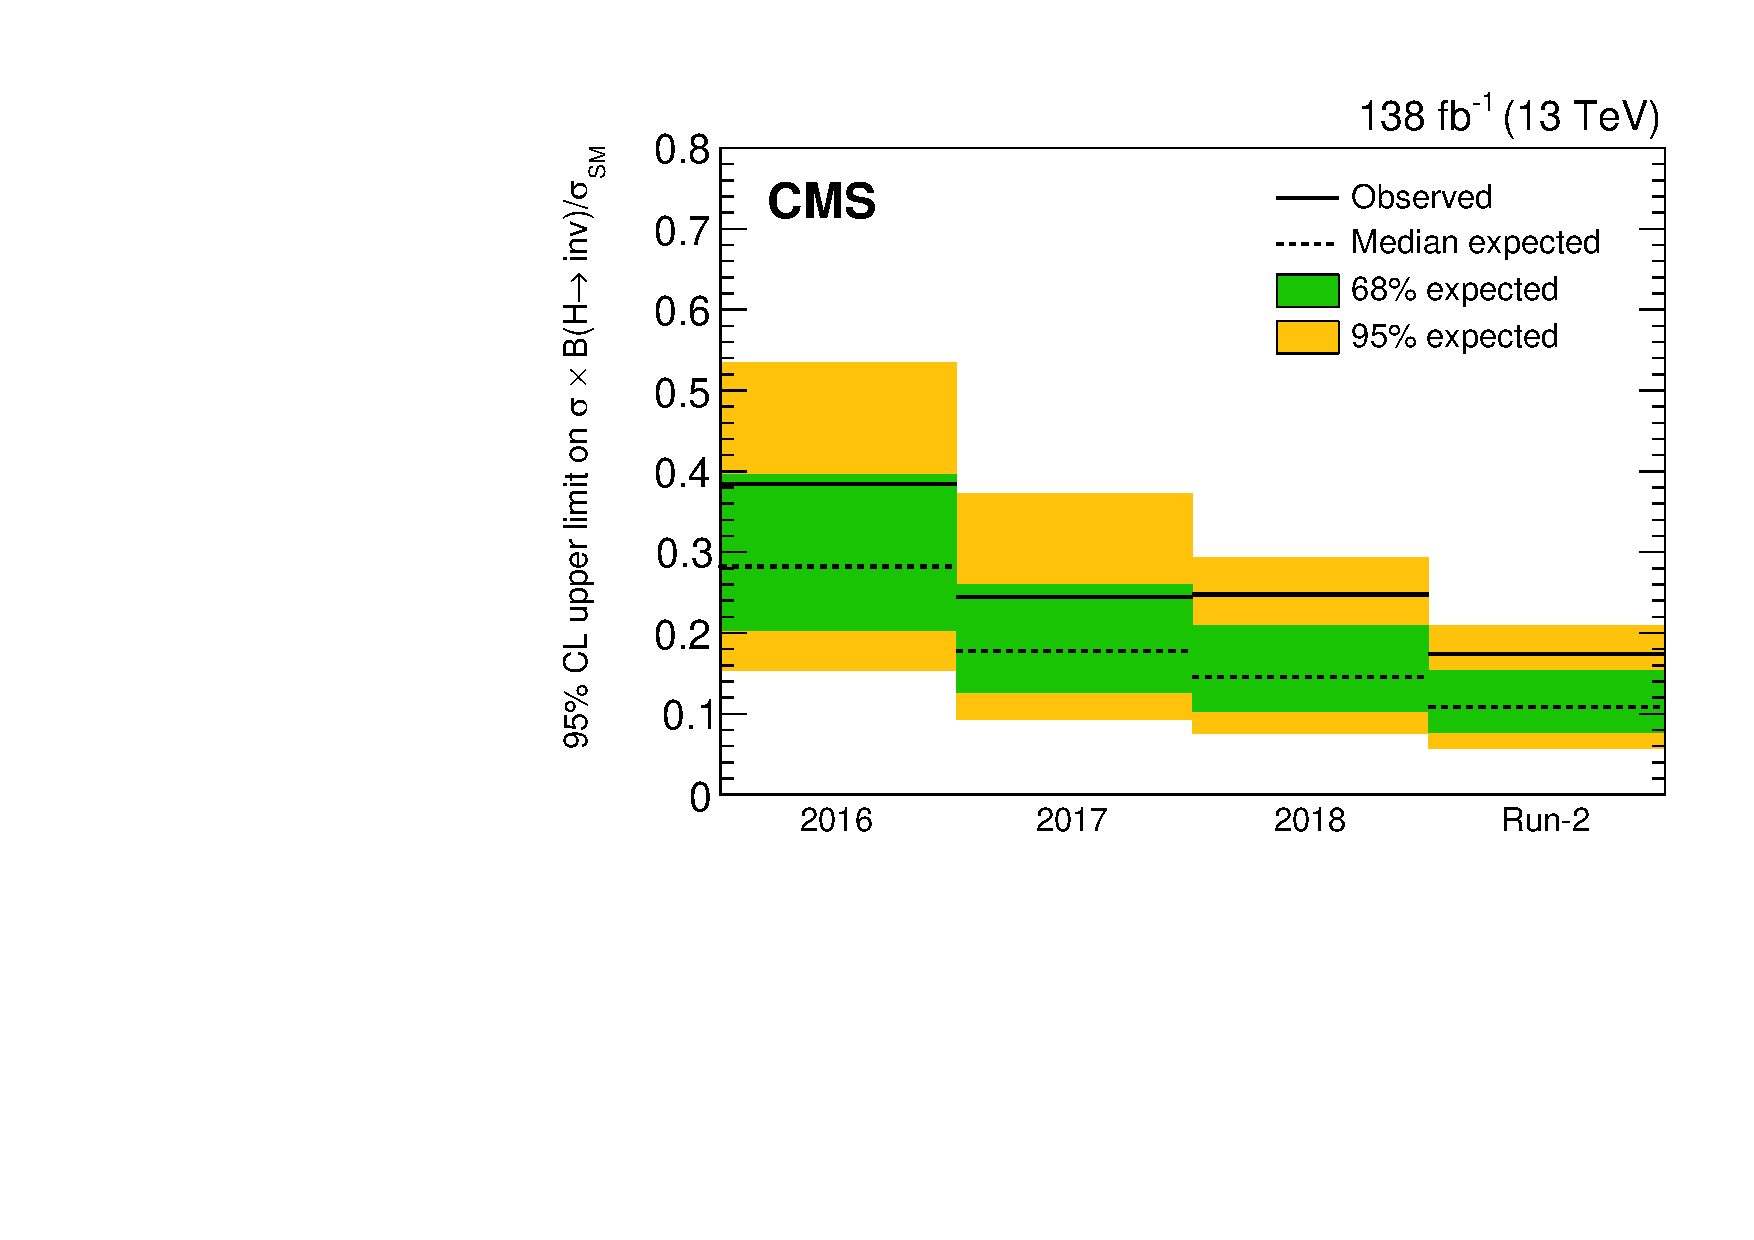
\includegraphics[width=0.7\textwidth]{from_paper/limits/limit_short.pdf}
    \caption{Observed and expected 95\% CL upper limits on $\sigmabr$ for all three data-taking years,
    together with the $1\sigma$ (green) and $2\sigma$ (yellow) uncertainty bands on the expected upper limits.
    The combination of 2016-2018 is also shown. These results assume a SM Higgs boson with a mass of 125.38 GeV.
    Figure taken from~\cite{VBFHinvAnalysisPaper}.}
    \label{fig:limit_short}
\end{figure}

\begin{table*}[h!]
    \centering
    \caption{The 95\% CL upper limits on ${\sigmabr}$, assuming an SM Higgs boson with a mass of 125.38 GeV. 
    The observed and median expected results are shown, along with the 68\% and 95\%  interquartile ranges for each 
    category and for the combinations.}
    \label{tab:limits}
    \def\arraystretch{1.05}
    \begin{tabular}{l c c c c}
       \hline
       Category & Observed & Median expected  & 65\% expected & 95\% expected \\
       \hline
          2012-2016  & 0.33  & 0.21  & [0.15,0.29]  & [0.11,0.39] \\ \\
    %    \hline
          VTR 2017  & 0.57  & 0.45  & [0.32,0.66]  & [0.24,0.94] \\ 
          VTR 2018  & 0.44  & 0.34  & [0.24,0.49]  & [0.18,0.69] \\ 
     VTR 2017 2018  & 0.40  & 0.28  & [0.20,0.40]  & [0.15,0.56] \\ \\
    %    \hline
          MTR 2017  & 0.25  & 0.19  & [0.14,0.28]  & [0.10,0.40] \\ 
          MTR 2018  & 0.24  & 0.15  & [0.11,0.22]  & [0.08,0.31] \\ 
     MTR 2017 2018  & 0.17  & 0.13  & [0.09,0.18]  & [0.07,0.25] \\ \\
    %    \hline
          all 2017  & 0.24  & 0.18  & [0.13,0.26]  & [0.09,0.37] \\ 
          all 2018  & 0.25  & 0.15  & [0.10,0.21]  & [0.08,0.29] \\ 
     all 2017 2018  & 0.18  & 0.12  & [0.08,0.17]  & [0.06,0.23] \\ \\
    %    \hline
              Run2  & 0.18  & 0.10  & [0.07,0.14]  & [0.05,0.20] \\ 
       \hline
    \end{tabular}
\end{table*}

\subsection{Upper bound on DM-nucleon interactions}

The upper limit on $\brinv$, obtained from combining the data taken between 2012 and 2018,
is interpreted in the context of Higgs-portal models of DM interactions, in which a stable 
DM particle couples to the SM Higgs boson. The interaction between a DM particle and an
atomic nucleus may be mediated by the exchange of a Higgs boson,
producing nuclear recoil signatures, such as those investigated by
direct-detection experiments. 

If the mass of the DM particle, $m_{DM}$, is smaller than half
of the mass of the Higgs boson, the Higgs boson invisible width ($\Gamma_{\text{inv}}$) can be translated,
within an effective field theory approach, into a spin-independent
DM-nucleon elastic scattering cross section, as outlined in
Ref.~\cite{Djouadi:2011aa}. This translation is performed assuming
that the DM candidate is either a scalar or a Majorana fermion, and
both the central value and the uncertainty of the dimensionless
nuclear form-factor $f_{N}$ are taken from the recommendations of
Ref.~\cite{Hoferichter:2017olk}. The conversion from \brinv to
$\Gamma_{\text{inv}}$ uses the relation ${\brinv = \Gamma_{\text{inv}}
/ (\Gamma_{\mathrm{SM}}+\Gamma_{\text{inv}})}$, where
$\Gamma_{\mathrm{SM}}$ is set to 4.07 MeV~\cite{Heinemeyer:2013tqa}.
The assumption of a vector DM candidate is not provided in the context of this analysis, since it
requires an extended dark Higgs sector, which may lead to
modifications of kinematic distributions assumed for the invisible
Higgs boson signal in this analysis.

Fig.~\ref{fig:DMlim} shows the 90\% CL upper
limits on the spin-independent DM-nucleon scattering cross section as
a function of $m_{\mathrm{DM}}$, for both the scalar and the fermion
DM scenarios. These limits are computed at 90\% CL so that they can
be compared with those from direct detection experiments such as
Xenon1T~\cite{Aprile:2018dbl}, Cresst-II~\cite{Angloher:2015ewa},
CDMSlite~\cite{Agnese:2015nto}, LUX~\cite{Akerib:2016vxi},
Panda-X 4T~\cite{PandaX-4T:2021bab}, and
DarkSide-50~\cite{Agnes:2018ves}, which provide the strongest
constraints in the $m_{\mathrm{DM}}$ range probed by this search. The
collider-based results complement the direct-detection experiments in
the range $m_{\mathrm{DM}}$ smaller than 12\,(6) GeV, assuming a
fermion (scalar) DM candidate.

\begin{figure}[htbp]
    \centering
    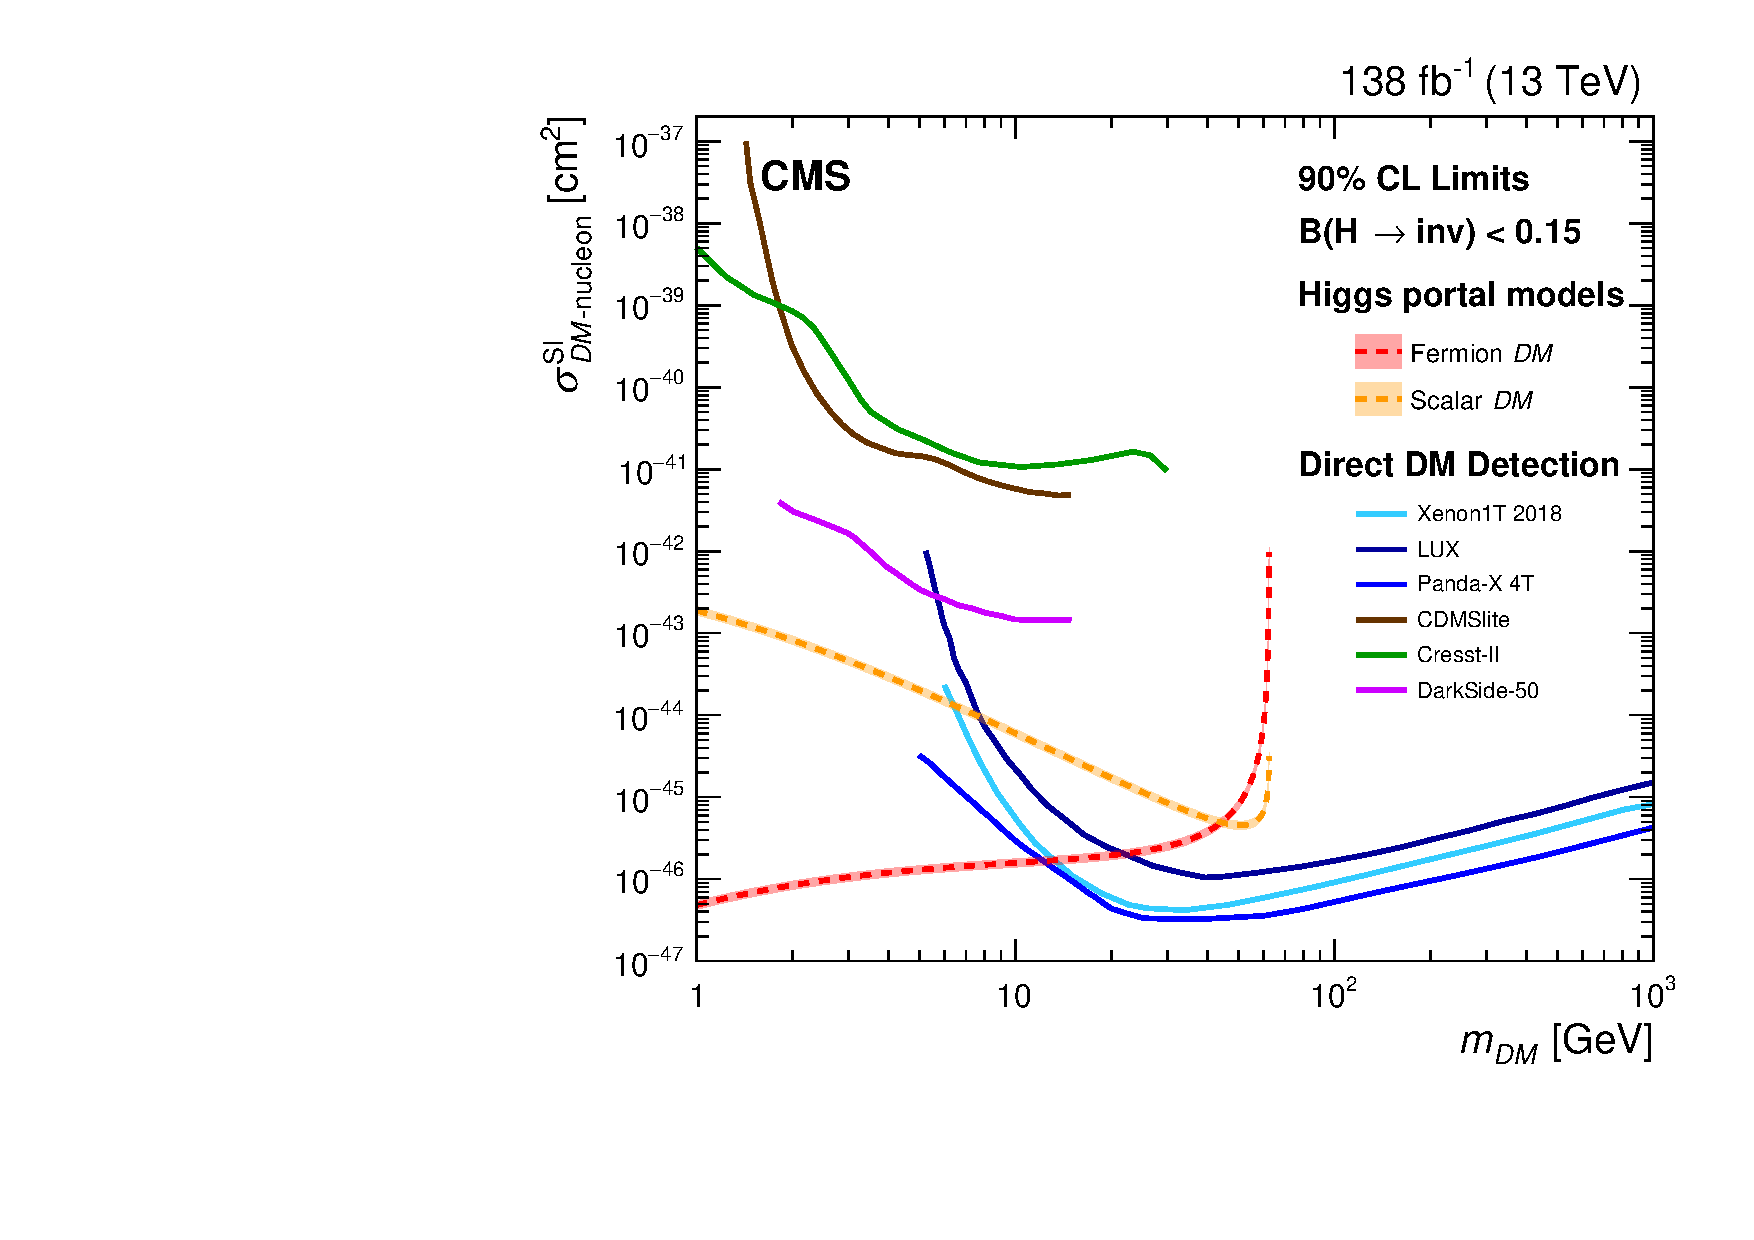
\includegraphics[width=0.8\textwidth]{from_paper/DM_nucleon_xs.pdf}
    \caption{The 90\% CL upper limits on the spin-independent DM-nucleon scattering cross 
    section in Higgs-portal models, assuming a scalar (dashed orange) or
    fermion (dashed red) DM candidate. Limits are computed as functions
    of $m_{\mathrm{DM}}$ and are compared to those from the
    Xenon1T~\cite{Aprile:2018dbl}, Cresst-II~\cite{Angloher:2015ewa},
    CDMSlite~\cite{Agnese:2015nto}, LUX~\cite{Akerib:2016vxi}, Panda-X
    4T~\cite{PandaX-4T:2021bab}, and DarkSide-50~\cite{Agnes:2018ves}
    experiments, which are shown as solid lines. Figure taken from~\cite{VBFHinvAnalysisPaper}.}
    \label{fig:DMlim}
\end{figure}